\documentclass[size=a4, parskip=half, titlepage=false, toc=flat, toc=bib, 12pt]{scrartcl}

\setuptoc{toc}{leveldown}

% Ajuste de las líneas y párrafos
\linespread{1.2}
\setlength{\parindent}{0pt}
\setlength{\parskip}{12pt}

% Español
\usepackage[spanish, es-tabla]{babel}

% Matemáticas
\usepackage{amsmath}
\usepackage{amsthm}

% Links
%\usepackage{hyperref}

% Fuentes
\usepackage{newpxtext,newpxmath}
\usepackage[scale=.9]{FiraMono}
\usepackage{FiraSans}
\usepackage[T1]{fontenc}

\defaultfontfeatures{Ligatures=TeX,Numbers=Lining}
\usepackage[activate={true,nocompatibility},final,tracking=true,factor=1100,stretch=10,shrink=10]{microtype}
\SetTracking{encoding={*}, shape=sc}{0}

\usepackage{graphicx}
\usepackage{float}

% Mejores tablas
\usepackage{booktabs}

\usepackage{adjustbox}

% COLORES

\usepackage{xcolor}

\definecolor{verde}{HTML}{007D51}
\definecolor{esmeralda}{HTML}{045D56}
\definecolor{salmon}{HTML}{FF6859}
\definecolor{amarillo}{HTML}{FFAC12}
\definecolor{morado}{HTML}{A932FF}
\definecolor{azul}{HTML}{0082FB}
\definecolor{error}{HTML}{b00020}

% ENTORNOS
\usepackage[skins, listings, theorems]{tcolorbox}

\newtcolorbox{recuerda}{
  enhanced,
%  sharp corners,
  frame hidden,
  colback=black!10,
	lefttitle=0pt,
  coltitle=black,
  fonttitle=\bfseries\sffamily\scshape,
  titlerule=0.8mm,
  titlerule style=black,
  title=\raisebox{-0.6ex}{\small RECUERDA}
}

\newtcolorbox{nota}{
  enhanced,
%  sharp corners,
  frame hidden,
  colback=black!10,
	lefttitle=0pt,
  coltitle=black,
  fonttitle=\bfseries\sffamily\scshape,
  titlerule=0.8mm,
  titlerule style=black,
  title=\raisebox{-0.6ex}{\small NOTA}
}

\newtcolorbox{error}{
  enhanced,
%  sharp corners,
  frame hidden,
  colback=error!10,
	lefttitle=0pt,
  coltitle=error,
  fonttitle=\bfseries\sffamily\scshape,
  titlerule=0.8mm,
  titlerule style=error,
  title=\raisebox{-0.6ex}{\small ERROR}
}

\newtcblisting{shell}{
  enhanced,
  colback=black!10,
  colupper=black,
  frame hidden,
  opacityback=0,
  coltitle=black,
  fonttitle=\bfseries\sffamily\scshape,
  %titlerule=0.8mm,
  %titlerule style=black,
  %title=Consola,
  listing only,
  listing options={
    style=tcblatex,
    language=sh,
    breaklines=true,
    postbreak=\mbox{\textcolor{black}{$\hookrightarrow$}\space},
    emph={jmml@UbuntuServer, jmml@CentOS},
    emphstyle={\bfseries},
  },
}

\newtcbtheorem[number within=section]{teor}{\small TEOREMA}{
  enhanced,
  sharp corners,
  frame hidden,
  colback=white,
  coltitle=black,
  fonttitle=\bfseries\sffamily,
  %separator sign=\raisebox{-0.65ex}{\Large\MI\symbol{58828}},
  description font=\itshape
}{teor}

\newtcbtheorem[number within=section]{prop}{\small PROPOSICIÓN}{
  enhanced,
  sharp corners,
  frame hidden,
  colback=white,
  coltitle=black,
  fonttitle=\bfseries\sffamily,
  %separator sign=\raisebox{-0.65ex}{\Large\MI\symbol{58828}},
  description font=\itshape
}{prop}

\newtcbtheorem[number within=section]{cor}{\small COROLARIO}{
  enhanced,
  sharp corners,
  frame hidden,
  colback=white,
  coltitle=black,
  fonttitle=\bfseries\sffamily,
  %separator sign=\raisebox{-0.65ex}{\Large\MI\symbol{58828}},
  description font=\itshape
}{cor}

\newtcbtheorem[number within=section]{defi}{\small DEFINICIÓN}{
  enhanced,
  sharp corners,
  frame hidden,
  colback=white,
  coltitle=black,
  fonttitle=\bfseries\sffamily,
  %separator sign=\raisebox{-0.65ex}{\Large\MI\symbol{58828}},
  description font=\itshape
}{defi}

\newtcbtheorem{ejer}{\small EJERCICIO}{
  enhanced,
  sharp corners,
  frame hidden,
  left=0mm,
  right=0mm,
  colback=white,
  coltitle=black,
  fonttitle=\bfseries\sffamily,
  %separator sign=\raisebox{-0.65ex}{\Large\MI\symbol{58828}},
  description font=\itshape,
  nameref/.style={},
}{ejer}

% CÓDIGO
\usepackage{listings}

% CABECERAS
\pagestyle{headings}
\setkomafont{pageheadfoot}{\normalfont\normalcolor\sffamily\small}
\setkomafont{pagenumber}{\normalfont\sffamily}

% ALGORITMOS
\usepackage[vlined,linesnumbered]{algorithm2e}

% Formato de los pies de figura
\setkomafont{captionlabel}{\scshape}
\SetAlCapFnt{\normalfont\scshape}
\SetAlgorithmName{Algoritmo}{Algoritmo}{Lista de algoritmos}

% BIBLIOGRAFÍA
%\usepackage[sorting=none]{biblatex}
%\addbibresource{bibliografia.bib}

\begin{document}

\renewcommand{\proofname}{\normalfont\sffamily\bfseries\small DEMOSTRACIÓN}

\title{Proyecto final\\
ShapeContext}
\subject{Visión por computador}
\author{Johanna Capote Robayna\\
    Guillermo Galindo Ortuño\\
    5 del Doble Grado en Informática y Matemáticas\\
    Grupo A}
\date{}
\publishers{\vspace{2cm}
\includegraphics[height=2.5cm]{UGR}\vspace{1cm}}
\maketitle

\newpage

\tableofcontents
\newpage

\section{Introducción}
En este proyecto vamos a implementar el descriptor \textit{ShapeContext}, presentado por Serge Belongie and Jitendra Malik en el paper <<Matching with Shape Contexts>> en el año 2000.

La principal idea del este algoritmo se basa construir un histograma basado en puntos en el sistema de coordenadas polares. Para cada punto, se obtiene la distancia y los ángulos euclidianos con respecto a otros puntos, se normalizan y se representa en las regiones del mapa el número de puntos de cada registro.

\begin{center}
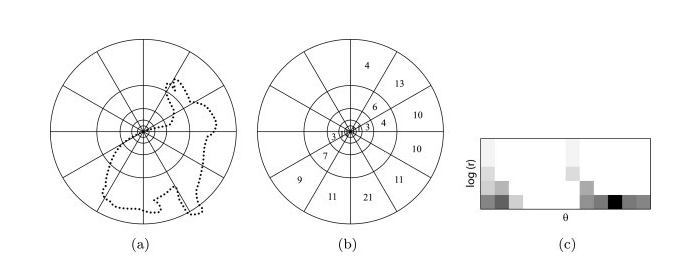
\includegraphics[height=6cm]{./img/intro}
\end{center}

Añadir información de que su utiliza principalmente para reconomiento de simbolos etc, y de sobre que lo vamos a probar etc.

\newpage

\section{Implementación}
Para implementar este algoritmo, se ha declarado una clase \verb|ShapeContext|. En el constructor declaramos los parámetros que determinan las regiones en las que se dividiremos la imagen. Es decir, el radio del circulo interior (\verb|r_inner|), el radio del último circulo exterior (\verb|r_outer|), el número de círculos concentricos (\verb|nbins_r|) y el número de regiones en las que se divide los círculos (\verb|nbins_theta|). Utilizamos los parámetros sugeridos en TODO.
%TODO Añadir referencias

\begin{verbatim}
    self.nbins_r = 5
    self.nbins_theta = 12
    self.r_inner = 0.1250
    self.r_outer = 2.0
\end{verbatim}

En primer lugar obtenemos los puntos del borde de la imagen que posteriormente le pasaremos al algoritmo para crear los histogramas. Para ello definimos la función \texttt{canny\_edge\_shape(self, img, max\_samples=100, t1=100, t2=200)}, que utiliza la implementación de \textit{OpenCV} del detector de bordes de \textit{Canny}, y devuelve hasta un máximo de 100 puntos distribuidos aleatorimente en el contorno.

\begin{verbatim}
edges = cv2.Canny(img, t1, t2)
    x, y = np.where(edges != 0)
    if x.shape[0] > max_samples:
        idx = np.random.choice(x.shape[0], max_samples, replace=False)
        x, y = x[idx], y[idx]
    shape = []
    for i in range(x.shape[0]):
        shape.append([x[i], y[i]])
    return shape
\end{verbatim}

A continuación, para construir los descriptores implementamos la función \texttt{compute(self, points)}. Esta será la encargada de recibir los puntos extraídos con la función anterior y construir un descriptor para cada uno.
\begin{enumerate}
\item En primer lugar calculamos la distancia entre todos los puntos dos a dos y la normalizamos por la media.

\begin{verbatim}
    t_points = len(points)
    r_array = cdist(points, points)
    r_array_n = r_array / r_array.mean()
\end{verbatim}

\item En segundo lugar creamos los registros y contamos el número de puntos que se encuentran encerrados en cada contenedor. Para ello creamos una matriz nula cuadrada de tamaño el número de puntos, que usaremos como contador para saber en que regiones se encuentra. En cada iteración comprobamos que los puntos sean menores que el el radio del círculo de la región que estamos testeando, si es menor, aumentamos el contador en uno.

Por ejemplo si nos encontramos en un espacio logaritmo con los siguientes intervalos.
logspace $= [\decimalpoint 0.1250, 0.2500, 0.5000, 1.0000, 2.0000]$ y tenemos la siguiente matriz de puntos:
$$\decimalpoint \begin{bmatrix}
0 & 1.3 \\
0.43 & 0
\end{bmatrix}$$
La matriz \verb|r_array_q| iría aumentando de la siguiente forma:
$$\decimalpoint \begin{bmatrix}
0 & 0 \\
0 & 0
\end{bmatrix} \stackrel{0 < 0.125}{\longrightarrow} \begin{bmatrix}
1 & 0 \\
0 & 1
\end{bmatrix} \stackrel{0 < 0.25}{\longrightarrow} \begin{bmatrix}
2 & 0 \\
0 & 2
\end{bmatrix} \stackrel{0 < 0.5}{\longrightarrow} \begin{bmatrix}
3 & 0 \\
1 & 3
\end{bmatrix} \stackrel{0.43 < 1.0}{\longrightarrow} \begin{bmatrix}
4 & 0 \\
2 & 4
\end{bmatrix} \stackrel{1.3 < 2.0}\rightarrow \begin{bmatrix}
5 & 1 \\
3 & 5
\end{bmatrix}$$

\begin{verbatim}
r_bin_edges =
    np.logspace(np.log10(r_inner), np.log10(r_outer), nbins_r)
r_array_q = np.zeros((t_points, t_points), dtype=int)
for m in xrange(self.nbins_r):
    r_array_q += (r_array_n < r_bin_edges[m])
\end{verbatim}

\item A continuación calculamos el ángulo entre los puntos, eliminamos posibles errores de redondeo y lo transformamos en un ángulo entre 0 y $2\pi$.
\begin{verbatim}
theta_array = cdist(points, points,
                lambda u, v:
                    math.atan2((v[1] - u[1]), (v[0] - u[0])))
theta_array[np.abs(theta_array) < 1e-7] = 0
theta_array_2 = theta_array + 2 * math.pi * (theta_array < 0)
\end{verbatim}
\item Fabricamos un histograma similar al de las distancias.
\begin{verbatim}
theta_array_q =
    (1 + np.floor(theta_array_2/(2*math.pi/self.nbins_theta)))
    .astype(int)
\end{verbatim}
\item Por último, al igual que con las distancias, fabricamos un contador para almacenar en que contenedor se encuentra el punto y almacenamos toda la información en un vector unidimensional, que será el descriptor asociado a dicho punto.
\begin{verbatim}
# building point descriptor based on angle and distance
nbins = self.nbins_theta * self.nbins_r
descriptor = np.zeros((t_points, nbins))
for i in range(t_points):
    sn = np.zeros((self.nbins_r, self.nbins_theta))
    for j in range(t_points):
        if (fz[i, j]):
            sn[r_array_q[i,j] - 1, theta_array_q[i,j] - 1] += 1
    descriptor[i] = sn.flatten()
\end{verbatim}
\end{enumerate}

El siguiente paso es establecer el coste de relacionar dos puntos, y como cada \textit{shape context} es en realidad una distribución representada como un histograma, es natural usar el test estadístico $\chi^2$
\[
C_{ij} = C(p_i,q_j) = \frac{1}{2} \sum_{k=1}^K \frac{[h_i(k) - h_j(k)]^2}{h_i(k) + h_j(k)},
\]
donde $h_i(k)$ y $h_j(k)$ son el valor del histograma asociado al k-ésimo contenedor de los punto $i$ y $j$ respectivamente. Este cálculo lo realiza la función \texttt{\_hist\_cost}:

\begin{verbatim}
def _hist_cost(self, hi, hj):
      cost = 0
      for k in range(self.nbins_theta * self.nbins_r):
          if (hi[k] + hj[k]):
              cost += ((hi[k] - hj[k])**2) / (hi[k] + hj[k])

      return cost * 0.5
\end{verbatim}

Ahora, dadas los descriptores asociados a todas los puntos de dos \textit{shapes} distintas, almacenamos todos los costes de asociar sus puntos dos a dos en una matriz. Antes de calcular el coste de dos descriptores, normalizamos los histogramas dividiendo por el total de puntos de cada forma respectivamente. Así, trabajamos con el porcentaje de puntos en cada contenedor, solventando el problema de que haya una gran diferencia de puntos en cada figura.

\begin{verbatim}
def _cost_matrix(self, P, Q, qlength=None):
      p, _ = P.shape
      q, _ = Q.shape
      C = np.zeros((p, q))
      for i in range(p):
          for j in range(q):
              C[i, j] = self._hist_cost(P[i]/p, Q[j]/q)

      return C
\end{verbatim}

A continuación necesitamos establecer una asignación entre los puntos de ambas formas que minimice la suma de los costes. Esto es un problema de asignación lineal, y para resolverlo utilizamos la implementación del \textit{algoritmo húngaro} disponible en la biblioteca \textit{Scipy}, \texttt{linear\_sum\_assignment}. Esta nos devuelve la asignación como dos vectores de índices, y con estos calculamos la suma de los costes asociados. Todo esto se encuentra implementado en el método \texttt{\_hungarian}, que devuelve el conjunto de indices y valor de la suma de los costes.

\begin{verbatim}
def _hungarian(self, cost_matrix):
      row_ind, col_ind = linear_sum_assignment(cost_matrix)
      total = cost_matrix[row_ind, col_ind].sum()
      indexes = zip(row_ind.tolist(), col_ind.tolist())
      return total, indexes
\end{verbatim}

Por último, la función \texttt{cost(self,P,Q)}, toma como argumentos los descriptores de cada imagen, calcula la matriz de costes y devuelve el coste mínimo calculado por el algoritmo húngaro.

Una vez implementado el algoritmo, podemos leer cualquier imagen y compararla con ella. La primera prueba que hemos realizado han sido con números, hemos implementados varias funciones para leer números de una imagen y tras calcular sus descriptores, le podemos pasar otra imagen con números de distinta fuente y comprobar que el algoritmo es capaz de establecer una conexión entre dos número de distinta fuente.

Para leer varios número de una misma imagen, hemos implementado la función \verb|parse_nums(sc, path)|, a la que se le pasa un objeto de la clase \verb|ShapeContext| y una ruta donde se encuentra la imagen. Esta función devuelve un vector de con los descriptores de cada punto.
\begin{enumerate}

\item En primer lugar, leemos la imagen, invertimos el color y ensanchamos los bordes, ya que los número que le pasamos a la imagen a veces son muy finos.

\begin{verbatim}
  img = cv2.imread(path, 0)
  img = cv2.bitwise_not(img)
  _, img = cv2.threshold(img, 254, 255, cv2.THRESH_BINARY)
  kernel = np.ones((2, 2), np.uint8)
  img = cv2.dilate(img, kernel, iterations=1)
\end{verbatim}

\item En segundo lugar, separamos los número uno a uno, para esto se define la función \verb|get_contour_bounding_rectangles(gray)| que devuelve un vector de tuplas de tamaño 4, una tupla por cada número de la imágen, donde cada una de las entradas de la tuplas se corresponde con las esquinas de un cuadrado que encierra el número.

\begin{verbatim}
  rois = get_contour_bounding_rectangles(img)
\end{verbatim}

\begin{figure}[H]
\centering
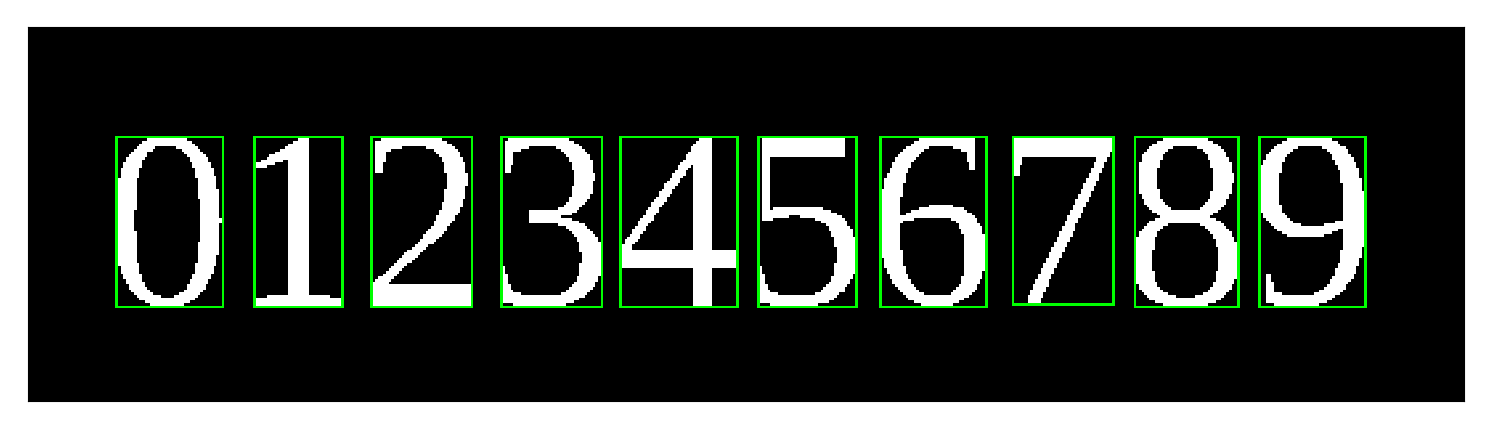
\includegraphics[height=4cm]{./img/numeros}
\caption{Ejemplo de como recuadra la función una imagen con números.}
\end{figure}

\item Creamos una lista de imágenes, en la que cada imagen solo aparezca una cifra, ya que ya sabemos las 4 esquinas de cada número. La imágenes las guardamos con el color original.

\begin{verbatim}
grayd = cv2.cvtColor(img.copy(), cv2.COLOR_GRAY2BGR)
  nums = []
  for r in rois:
      grayd = cv2.rectangle(grayd, (r[0], r[1]), (r[2], r[3]),
                                                (0, 255, 0), 1)
      nums.append((r[0], r[1], r[2], r[3]))
\end{verbatim}

\item A continuación por cada carácter calculamos el descriptor. Llamando primero a la función \verb|canny_edge_shape| que obtiene los puntos y posteriormente se le pasalos puntos a la función \verb|compute| para construir el descriptor correspondiente a los puntos de ese carácter. Antes de calcular los descriptores, ordenamos las imágenes que corresponden a cada carácter por su esquina superior izquierda, así el primer descriptor corresponderá con el primer carácter que aparezca.

\begin{verbatim}
  nums = sorted(nums, key=lambda x: x[0])
  descs = []
  for i, r in enumerate(nums):
      if img[r[1]:r[3], r[0]:r[2]].mean() < 50:
          continue
      points = sc.canny_edge_shape(img[r[1]:r[3], r[0]:r[2]])
      descriptor = sc.compute(points)

      descs.append(descriptor)
  return np.array(descs)
\end{verbatim}

\end{enumerate}
Por último para establecer las correspondencias entre caracteres se utiliza la función \verb|match(base, current)|

\newpage

\section{Análisis de resultados}
En primer lugar probamos el algoritmo pasandole como base todos los números (del 0 al 9) y como prueba introducimos una serie de números aleatorios con distintas fuentes.

\begin{figure}[H]
\centering
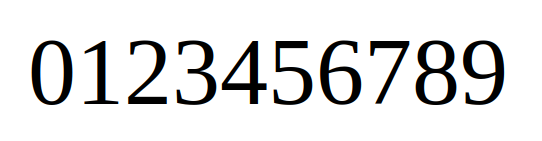
\includegraphics[width=8cm]{./img/base}
\caption{Números utilizados como base}
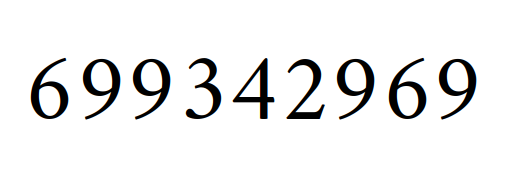
\includegraphics[width=8cm]{./img/telefono}
\caption{Números de otra fuente distinta a la fuente de los números base}
\end{figure}

Como resultado obtenemos la salida:

\begin{figure}[H]
\centering
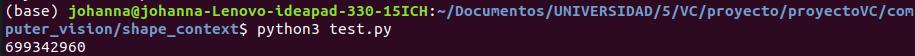
\includegraphics[width=15cm]{./img/restelefono}
\caption{Resultado de ejecutar el algoritmo con las dos imágenes anteriores.}
\end{figure}

Vemos que el único número que no ha detectado el bien es

Utilizando la misma base que el ejemplo anterior, probamos otros números con otra fuente.
\begin{figure}[H]
\centering
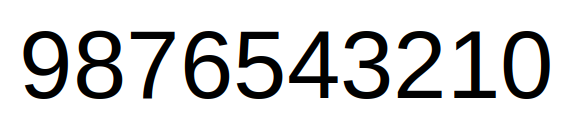
\includegraphics[width=8cm]{./img/otrafuente}
\caption{Números de otra fuente distinta a la fuente de los números base}
\end{figure}
Como resultado obtenemos:

\begin{figure}[H]
\centering
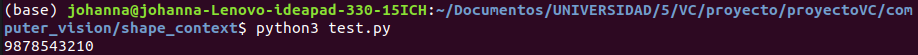
\includegraphics[width=15cm]{./img/resotra}
\caption{Resultado de ejecutar el algoritmo con la imagen anterior y la imagen base.}
\end{figure}

Probamos con números escritos a mano:
\begin{figure}[H]
\centering
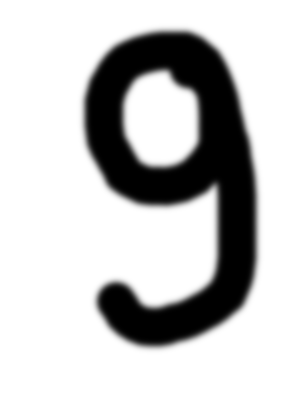
\includegraphics[width=8cm]{./img/9}
\caption{Números 9 escrito a mano}
\end{figure}
\begin{figure}[H]
\centering
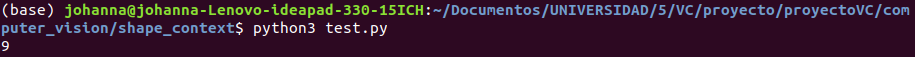
\includegraphics[width=8cm]{./img/res9}
\caption{Resultado del número anterior comparado con los números base.}
\end{figure}

A continuación vamos a realizar pruebas con letras en vez de números, para ello utilizaremos un abecedario y posteriormente introduciremos palabras para comprobar como de bien las reconoce.

\begin{figure}[H]
\centering
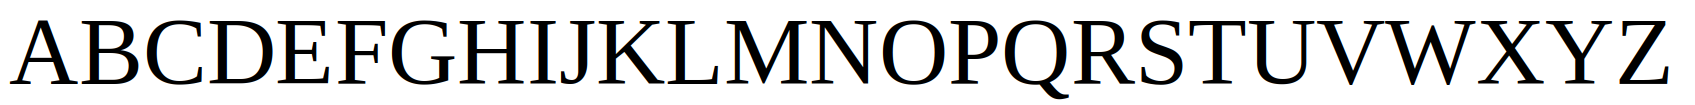
\includegraphics[width=15cm]{./img/ABC}
\caption{Alfabeto utilizado como base}

\includegraphics[width=8cm]{./img/JOHANNA}
\caption{Palabra utilizada para comprobar la eficiencia del algoritmo con letras.}
\end{figure}

El resultado es el siguiente:
\begin{figure}[H]
\centering
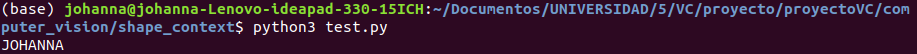
\includegraphics[width=15cm]{./img/resjohanna}
\caption{Resultado de ejecutar el algoritmo con la imagen anterior y la imagen base.}
\end{figure}

Probamos con otras palabras con otro tipo de fuente:
\begin{figure}[H]
\centering

\includegraphics[width=8cm]{./img/GUILLERMO}
\caption{Resultado de ejecutar el algoritmo con la imagen anterior y la imagen base.}
\end{figure}

Como resultado obtenemos:

\begin{figure}[H]
\centering
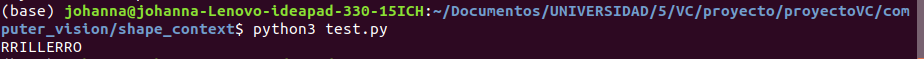
\includegraphics[width=15cm]{./img/resguillermo}
\caption{Resultado de ejecutar el algoritmo con la imagen anterior y la imagen base.}
\end{figure}

Hacemos más pruebas con otras letras más deformadas, por ejemplo:

\begin{figure}[H]
\centering

\includegraphics[width=4cm]{./img/AM}
\caption{Letra A deformada.}
\end{figure}

Y obtenemos el resultado correcto:
\begin{figure}[H]
\centering
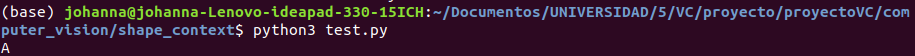
\includegraphics[width=15cm]{./img/resa}
\caption{Resultado de ejecutar el algoritmo con la imagen anterior y la imagen base.}
\end{figure}

%printbibliography

\end{document}
